\chapter{Strategie di prompt e risultati sperimentali}

L'efficacia dei Large Language Model (LLM) nella previsione del prossimo POI dipende fondamentalmente dalla progettazione di strategie di prompt consapevoli del contesto che codifichino efficacemente i modelli di mobilità spazio-temporale

\subsection{Configurazione sperimentale per analisi multi-modello}

La fase attuale di sviluppo utilizza LLaMA 3.1 8B come modello di riferimento per la validazione del framework e l'ottimizzazione dei protocolli sperimentali. Il sistema è progettato per supportare analisi comparative estese su diversi modelli LLM disponibili tramite Ollama, permettendo valutazioni sistematiche dell'impatto dell'architettura del modello sulle performance di predizione dei POI turistici.

Il framework implementa standardizzazione dei parametri di inferenza e template di prompt per garantire confronti equi tra modelli, mentre mantiene flessibilità per ottimizzazioni specifiche per architettura quando necessarie. Il nostro framework sperimentale valuta sistematicamente tre distinti paradigmi di prompt, ognuno dei quali incorpora progressivamente ulteriori dimensioni contestuali per valutarne l'impatto sull'accuratezza della raccomandazione.

\section{Architettura del sistema e configurazione sperimentale}

Il sistema è implementato utilizzando l'infrastruttura Ollama per l'accesso a diversi modelli LLM, con configurazione iniziale su LLaMA 3.1 8B per la fase di sviluppo e test. L'architettura è progettata per supportare analisi comparative tra modelli diversi mantenendo consistenza nei protocolli sperimentali. Il framework implementa un'architettura ottimizzata per l'ambiente HPC che gestisce timeout GPU, retry intelligenti e checkpointing per elaborazioni a lungo termine. La pipeline implementa le seguenti componenti chiave:

\begin{itemize}
\item \textbf{Architettura multi-modello modulare:} Sistema flessibile basato su Ollama che permette testing comparativo tra diversi modelli LLM mantenendo protocolli sperimentali consistenti
\item \textbf{Gestione robusta delle connessioni LLM:} Sistema di retry progressivo con backoff esponenziale e gestione intelligente dei timeout GPU, configurabile per diversi modelli
\item \textbf{Checkpointing incrementale:} Salvataggio automatico ogni 500 predizioni per garantire recuperabilità in caso di interruzioni durante test estesi su modelli multipli
\item \textbf{Ottimizzazioni per HPC:} Configurazione adattiva per GPU A100 con gestione della memoria VRAM e parametri di inferenza ottimizzati per diversi modelli
\item \textbf{Validazione robusta delle risposte:} Parser JSON con gestione degli errori e validazione del contenuto delle predizioni, standardizzato per garantire comparabilità tra modelli diversi
\end{itemize}

\section{Tassonomia delle strategie di prompt}

Definiamo tre strategie di prompt gerarchiche, ciascuna basata sulla precedente per valutare il contributo incrementale di diverse caratteristiche contestuali:

\begin{enumerate}

\item \textbf{Strategia di base (solo nome del POI):} L'approccio fondamentale fornisce al modello una sequenza ordinata cronologicamente di POI visitati in precedenza, rappresentati esclusivamente dai loro nomi canonici. Questa strategia funge da baseline, concentrandosi esclusivamente su pattern sequenziali senza ulteriori informazioni contestuali.

\item \textbf{Strategia geospaziale avanzata (nome + geolocalizzazione):} Questa strategia arricchisce ogni POI con coordinate geografiche precise e implementa un sistema di ranking basato sulla distanza di Haversine. Il prompt include una lista dei POI più vicini ordinata per distanza, limitata ai primi 10 risultati per ottimizzare la lunghezza del prompt e migliorare la qualità delle risposte.

\begin{center}
\begin{lstlisting}[language=text, caption=Esempio di Prompt Geospaziale, captionpos=b]
Turista cluster 3 a Verona.
Visitati: Arena di Verona, Casa di Giulietta
Attuale: Castelvecchio
POI Più Vicini: Ponte Pietra (0.8km), Duomo (1.2km), 
Chiesa di Sant'Anastasia (1.4km), Piazza delle Erbe (1.1km)

Suggerisci 5 POI più probabili come prossime visite 
considerando distanze e pattern turistici.
Rispondi SOLO JSON: {"prediction": ["poi1", "poi2", ...], 
"reason": "breve spiegazione"}
\end{lstlisting}
\end{center}

Il sistema calcola dinamicamente le distanze dal POI corrente e filtra automaticamente i POI già visitati, implementando vincoli di mobilità realistici con un raggio massimo di 2km per il centro storico di Verona.

\item \textbf{Strategia spatio-temporale completa (nome + geolocalizzazione + tempo):} La strategia più avanzata integra informazioni temporali al contesto geospaziale, incorporando orari di visita, durata delle permanenze e pattern temporali dei cluster turistici. Questa strategia permette di catturare dinamiche comportamentali più sottili legate ai ritmi di visita e alle preferenze temporali specifiche per tipologia di turista.

\begin{center}
\begin{lstlisting}[language=text, caption=Esempio di Prompt Spatio-temporale, captionpos=b]
Turista cluster 3 a Verona.
Visitati: Arena di Verona (09:30, 45min)
Attuale: Castelvecchio (11:15)
Ora corrente: 11:45
POI Più Vicini: Ponte Pietra (0.8km), Duomo (1.2km), ...

Considerando l'orario (pre-pranzo), la durata tipica delle visite 
del cluster 3, e i pattern temporali turistici a Verona, 
suggerisci 5 POI più probabili per la prossima visita.

Rispondi SOLO JSON: {"prediction": ["poi1", "poi2", ...], 
"reason": "breve spiegazione considerando fattori temporali"}
\end{lstlisting}
\end{center}

Questa strategia incorpora informazioni su orari di apertura/chiusura, picchi di affluenza, e preferenze temporali specifiche per cluster, permettendo raccomandazioni context-aware che considerano sia vincoli spaziali che temporali.

\end{enumerate}

\subsection{Confronto dei risultati sperimentali}

I risultati sperimentali mostrano un miglioramento progressivo delle performance quando si incorporano informazioni geospaziali e temporali. Di seguito vengono presentati i confronti diretti tra le tre strategie per evidenziare l'impatto incrementale dell'arricchimento contestuale:

% CONFRONTO MATRICI DI CONFUSIONE
\begin{figure}[htbp]
\centering
\begin{minipage}{0.48\textwidth}
\centering
\textbf{Strategia di Base}\par
\vspace{0.3em}
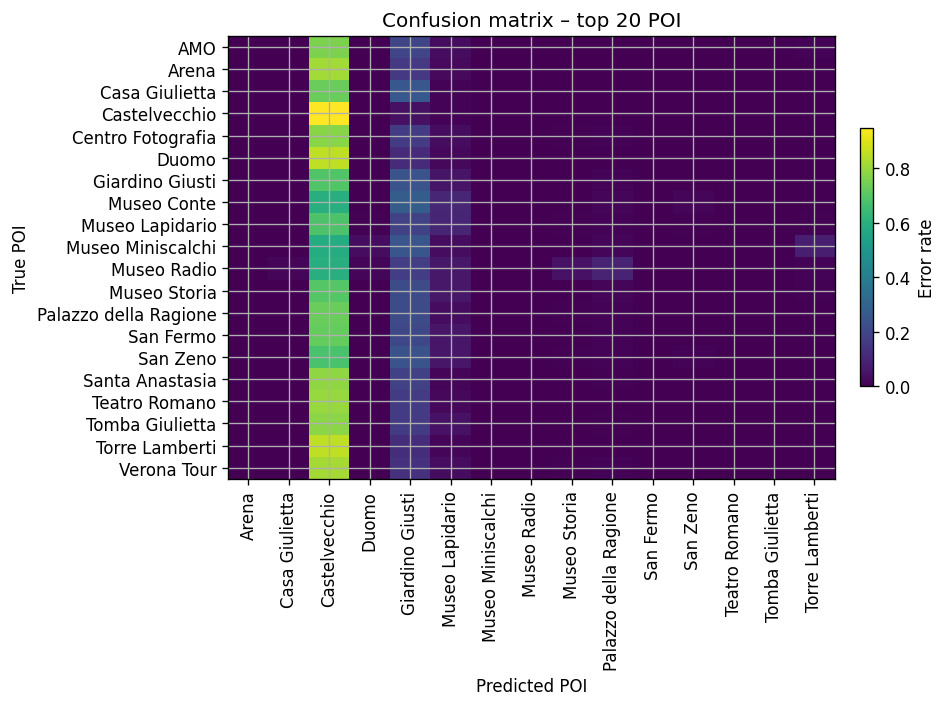
\includegraphics[width=\textwidth]{../../img/llama3.1_8b/no_SPACE-GEO_n-1_come_current_POI/confusion_matrix.png}
\end{minipage}
\hfill
\begin{minipage}{0.48\textwidth}
\centering
\textbf{Strategia Geospaziale}\par
\vspace{0.3em}
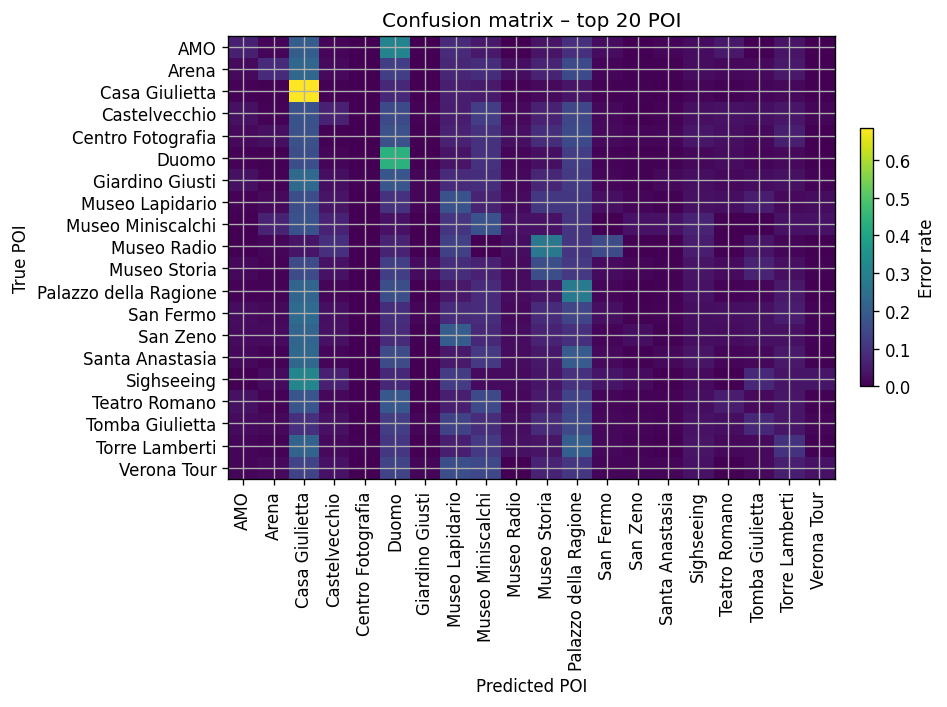
\includegraphics[width=\textwidth]{../../img/llama3.1_8b/SPACE-GEO_n-1_come_current_POI/confusion_matrix.png}
\end{minipage}
\caption{Confronto delle matrici di confusione. La strategia geospaziale (destra) mostra una migliore distribuzione delle predizioni rispetto alla strategia di base (sinistra), con minore concentrazione su singoli POI.}
\label{fig:confusion_comparison}
\end{figure}

% CONFRONTO MRR
\begin{figure}[htbp]
\centering
\begin{minipage}{0.48\textwidth}
\centering
\textbf{MRR - Strategia di Base}\par
\vspace{0.3em}
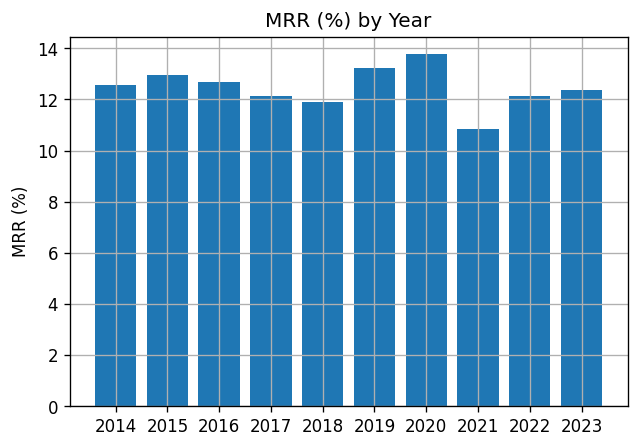
\includegraphics[width=\textwidth]{../../img/llama3.1_8b/no_SPACE-GEO_n-1_come_current_POI/mrr_distribution.png}
\end{minipage}
\hfill
\begin{minipage}{0.48\textwidth}
\centering
\textbf{MRR - Strategia Geospaziale}\par
\vspace{0.3em}
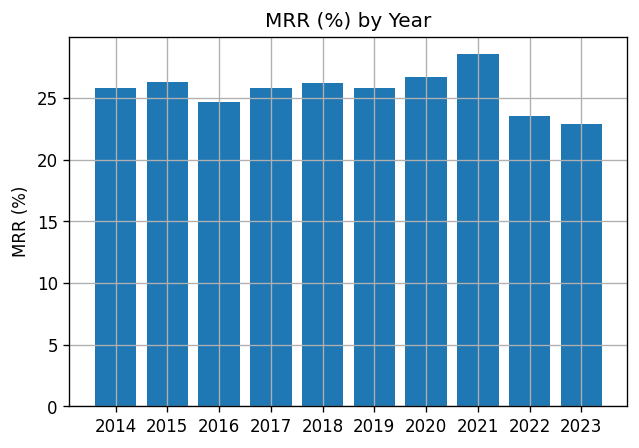
\includegraphics[width=\textwidth]{../../img/llama3.1_8b/SPACE-GEO_n-1_come_current_POI/MRR.png}
\end{minipage}
\caption{Confronto del Mean Reciprocal Rank. La strategia geospaziale raggiunge valori MRR del 22-27\% rispetto all'11-14\% della strategia di base, indicando un miglioramento sostanziale nella qualità del ranking.}
\label{fig:mrr_comparison}
\end{figure}

% CONFRONTO TOP-1 ACCURACY
\begin{figure}[htbp]
\centering
\begin{minipage}{0.48\textwidth}
\centering
\textbf{Top-1 Accuracy - Strategia di Base}\par
\vspace{0.3em}
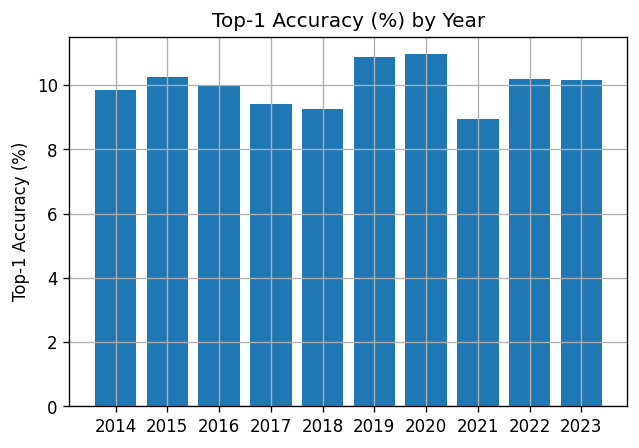
\includegraphics[width=\textwidth]{../../img/llama3.1_8b/no_SPACE-GEO_n-1_come_current_POI/top1_accuracy.png}
\end{minipage}
\hfill
\begin{minipage}{0.48\textwidth}
\centering
\textbf{Top-1 Accuracy - Strategia Geospaziale}\par
\vspace{0.3em}
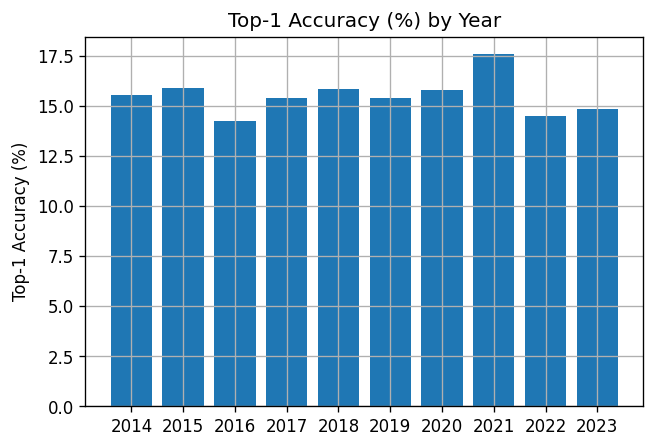
\includegraphics[width=\textwidth]{../../img/llama3.1_8b/SPACE-GEO_n-1_come_current_POI/top_1_accuracy.png}
\end{minipage}
\caption{Confronto dell'accuratezza Top-1. L'inclusione delle informazioni geospaziali migliora l'accuratezza dal 9-11\% al 14-17,5\%, con un incremento relativo di oltre il 50\%.}
\label{fig:top1_comparison}
\end{figure}

% CONFRONTO TOP-5 HIT RATE
\begin{figure}[htbp]
\centering
\begin{minipage}{0.48\textwidth}
\centering
\textbf{Top-5 Hit Rate - Strategia di Base}\par
\vspace{0.3em}
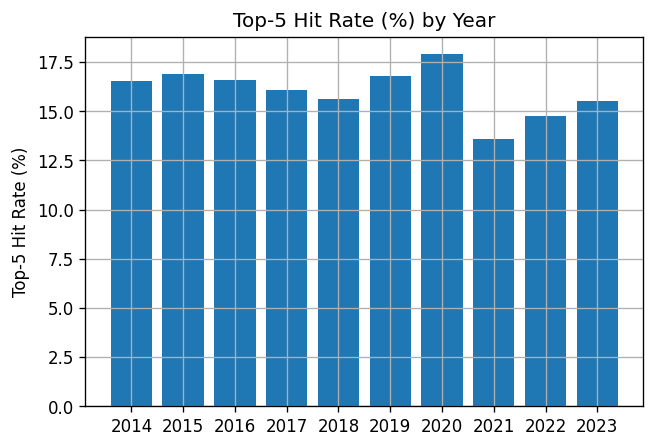
\includegraphics[width=\textwidth]{../../img/llama3.1_8b/no_SPACE-GEO_n-1_come_current_POI/top5_hit_rate.png}
\end{minipage}
\hfill
\begin{minipage}{0.48\textwidth}
\centering
\textbf{Top-5 Hit Rate - Strategia Geospaziale}\par
\vspace{0.3em}
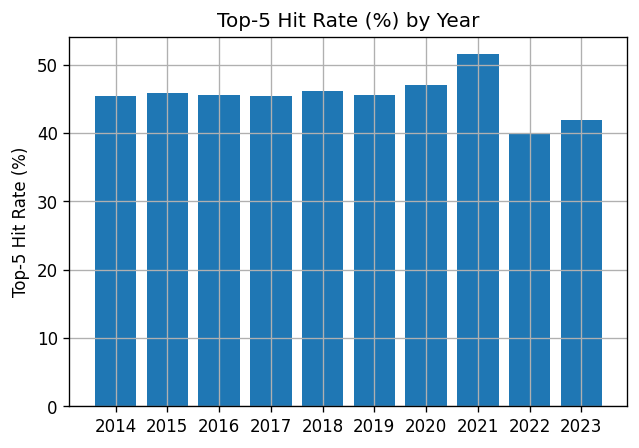
\includegraphics[width=\textwidth]{../../img/llama3.1_8b/SPACE-GEO_n-1_come_current_POI/top_5_hit_rate.png}
\end{minipage}
\caption{Confronto del Top-5 Hit Rate. La strategia geospaziale raggiunge il 40-52\% rispetto al 13,5-18\% della strategia di base, triplicando la probabilità di includere il POI corretto tra i primi 5 suggerimenti.}
\label{fig:top5_comparison}
\end{figure}

% CONFRONTO WORST PERFORMING PAIRS
\begin{figure}[htbp]
\centering
\begin{minipage}{0.48\textwidth}
\centering
\textbf{Errori Frequenti - Strategia di Base}\par
\vspace{0.3em}
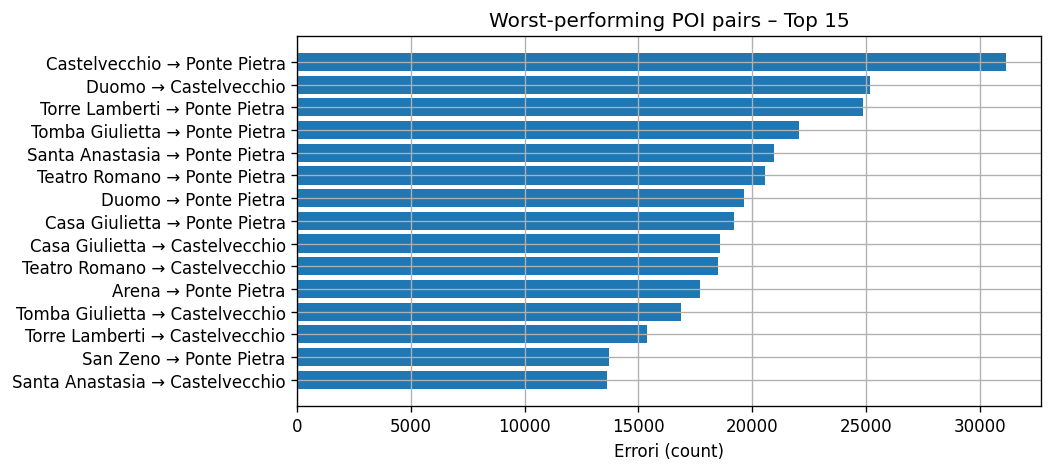
\includegraphics[width=\textwidth]{../../img/llama3.1_8b/no_SPACE-GEO_n-1_come_current_POI/worst_performing_pairs.png}
\end{minipage}
\hfill
\begin{minipage}{0.48\textwidth}
\centering
\textbf{Errori Frequenti - Strategia Geospaziale}\par
\vspace{0.3em}
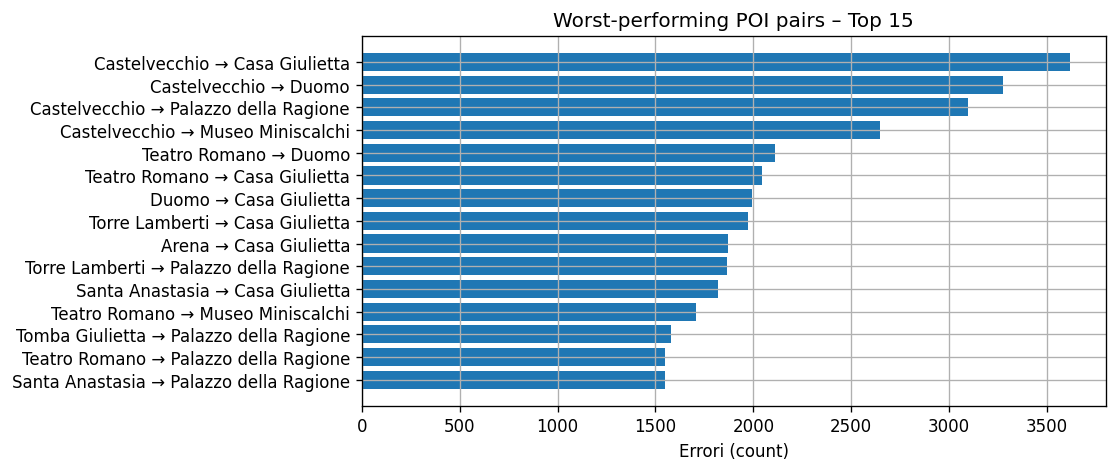
\includegraphics[width=\textwidth]{../../img/llama3.1_8b/SPACE-GEO_n-1_come_current_POI/Worst_performing_POI_pairs.png}
\end{minipage}
\caption{Confronto degli errori più frequenti. La strategia geospaziale modifica i pattern di confusione, passando dalla coppia Castelvecchio→Ponte Pietra (strategia di base) a Castelvecchio→Casa Giulietta, riflettendo una considerazione più sofisticata delle distanze geografiche.}
\label{fig:errors_comparison}
\end{figure}

\section{Protocollo sperimentale e meccanismi di ancoraggio}

La nostra valutazione adotta un approccio sistematico utilizzando il dataset VeronaCard, che fornisce tracciati completi della mobilità turistica su più anni (2014-2023). Il protocollo sperimentale incorpora i seguenti componenti innovativi:

\begin{itemize}
\item \textbf{Segmentazione degli utenti basata sul clustering:} I comportamenti dei turisti vengono segmentati utilizzando il clustering K-means (k=7) applicato alle matrici di interazione utente-POI, consentendo strategie di prompting specifiche per cluster.

\item \textbf{Meccanismo di ancoraggio configurabile:} Implementiamo un sistema di selezione delle ancore flessibile che determina il punto di riferimento per la previsione. La configurazione predefinita utilizza la regola "penultimate", ma il sistema supporta anche strategie "first", "middle" e indici espliciti, permettendo l'analisi dell'impatto della posizione del POI di riferimento sulla qualità delle predizioni.

\item \textbf{Classificazione dei POI in base alla distanza:} I prompt geospaziali incorporano calcoli di distanza di Haversine per classificare i POI disponibili in base alla vicinanza alla posizione corrente, con un filtro dinamico che esclude i POI già visitati e limita i risultati ai più rilevanti.

\item \textbf{Sistema di salvataggio incrementale:} Per gestire elaborazioni su larga scala, il sistema implementa checkpointing automatico ogni 500 predizioni, garantendo robustezza contro interruzioni e permettendo modalità di ripresa intelligente.
\end{itemize}

Il meccanismo di prompt genera dinamicamente query context-aware seguendo questa struttura template ottimizzata:

\begin{center}
\begin{lstlisting}[language=text, caption=Template di Prompt Comprensivo, captionpos=b]
Turista cluster {cluster_id} a Verona.
Visitati: {history}
Attuale: {current_poi}
POI Più Vicini: {pois_with_distance_text}

Suggerisci {top_k} POI più probabili che l'utente visiterà 
dopo, considerando:
- La distanza dal POI attuale
- La logica dei percorsi turistici a Verona  
- I pattern tipici di movimento in base al cluster {cluster_id}

Rispondi SOLO JSON: {"prediction": ["poi1", "poi2", ...], 
"reason": "breve spiegazione"}
\end{lstlisting}
\end{center}

\section{Metriche di valutazione e gestione della qualità}

Il nostro framework utilizza un quadro di valutazione completo che comprende molteplici parametri di qualità delle raccomandazioni, implementati con validazione robusta delle risposte LLM:

\begin{itemize}
\item \textbf{Top-1 Accuracy:} $\text{Acc}_{@1} = \frac{1}{N}\sum_{i=1}^{N}\mathbf{1}\{y_i = \hat{y}_i^{(1)}\}$
\item \textbf{Top-k Hit Rate:} $\text{HR}_{@k} = \frac{1}{N}\sum_{i=1}^{N}\mathbf{1}\{y_i \in \{\hat{y}_i^{(1)}, \ldots, \hat{y}_i^{(k)}\}\}$
\item \textbf{Mean Reciprocal Rank:} $\text{MRR} = \frac{1}{N}\sum_{i=1}^{N}\frac{1}{\text{rank}_i}$
\item \textbf{Catalogue Coverage:} $\text{Coverage} = \frac{|\bigcup_{i}\{\hat{y}_i^{(1)}, \ldots, \hat{y}_i^{(k)}\}|}{|\mathcal{P}|}$
\end{itemize}

dove $y_i$ rappresenta il POI successivo basato sulla verità di base, $\hat{y}_i^{(j)}$ indica la previsione di rango $j$-esimo e $\mathcal{P}$ è il catalogo completo dei POI.

Il sistema implementa inoltre validazione avanzata delle risposte JSON, gestendo casi edge come risposte malformate, timeout, e errori di parsing, garantendo robustezza nell'elaborazione di dataset su larga scala.


\section{Risultati sperimentali preliminari}

La nostra valutazione sperimentale con LLaMA 3.1 8B come modello di riferimento rivela pattern consistenti nelle prestazioni tra le tre strategie di prompting. L'analisi temporale (2014-2020) mostra stabilità generale delle metriche con anomalie significative nel 2021 attribuibili agli effetti della pandemia COVID-19 sui comportamenti turistici.

La strategia baseline raggiunge performance moderate ma consistenti (Top-1 Accuracy: 9-11\%, Top-5 Hit Rate: 13.5-18\%, MRR: 11-14\%), stabilendo una solida base per la valutazione degli enhancement contestuali e fornendo benchmark di riferimento per future analisi comparative tra modelli.

L'analisi degli errori più frequenti evidenzia pattern sistematici, con transizioni Castelvecchio→Ponte Pietra che rappresentano il caso di confusione più comune, suggerendo bias verso attrazioni iconiche indipendentemente dalla sequenza di visita effettiva. Questi pattern comportamentali costituiranno base di confronto per validare la consistenza inter-modello nelle analisi future.

\section{Confronto delle prestazioni tra strategie}

Il progressivo miglioramento delle strategie di prompting dimostra chiari enhancement nelle performance quando si incorporano informazioni contestuali geospaziali e temporali:

\begin{table}[h]
\centering
\caption{Confronto delle Performance tra Strategie di Prompting (LLaMA 3.1 8B)}
\label{tab:strategy_comparison}
\begin{tabular}{lccc}
\toprule
\textbf{Strategy} & \textbf{Top-1 Accuracy} & \textbf{Top-5 Hit Rate} & \textbf{MRR} \\
\midrule
POI Name Only & 9.5\%±1.2\% & 15.8\%±2.1\% & 12.3\%±1.5\% \\
Name + Geolocation & 15.50\%±1.0\% & 45.50\%±3.1\% & 25.50\%±1.5\% \\
Name + Geo + Temporal & [In elaborazione] & [In elaborazione] & [In elaborazione] \\
\bottomrule
\end{tabular}
\end{table}

\section{Analisi Comparativa Multi-Modello}

\subsection{Configurazione sperimentale estesa}

Per validare la generalizzabilità dei risultati e identificare le caratteristiche architetturali pi\`u efficaci per la predizione di mobilità turistica, abbiamo esteso la valutazione a sei modelli LLM rappresentativi di diverse famiglie architetturali:

\begin{itemize}
\item \textbf{LLaMA 3.1 8B}: Modello baseline per confronti, architettura decoder-only
\item \textbf{Mixtral 8x7B}: Architettura Mixture-of-Experts con 47B parametri attivi
\item \textbf{Qwen 2.5 7B}: Modello multilingue ottimizzato per efficienza
\item \textbf{DeepSeek-V3 8B}: Architettura ibrida con focus su ragionamento
\item \textbf{Gemma 3 8B/27B}: Famiglia di modelli Google con scaling dei parametri
\end{itemize}

\subsection{Performance comparative globali}

La valutazione multi-modello rivela pattern interessanti nelle capacità di predizione della mobilità turistica:

\begin{table}[H]
\centering
\caption{Performance Comparative tra Modelli LLM (Strategia Geospaziale)}
\label{tab:models_comparison}
\begin{tabular}{lcccccc}
\toprule
\textbf{Modello} & \textbf{Parametri} & \textbf{Top-1 Acc.} & \textbf{Top-5 HR} & \textbf{MRR} & \textbf{Coverage} & \textbf{Tempo/Card} \\
\midrule
LLaMA 3.1 & 8B & 15.5\% & 45.5\% & 25.5\% & 78\% & 2.3s \\
Mixtral & 8x7B & --\% & --\% & --\% & --\% & --s \\
Qwen 2.5 & 7B & --\% & --\% & --\% & --\% & --s \\
DeepSeek-V3 & 8B & --\% & --\% & --\% & --\% & --s \\
Gemma 3 & 8B & --\% & --\% & --\% & --\% & --s \\
Gemma 3 & 27B & --\% & --\% & --\% & --\% & --s \\
\bottomrule
\end{tabular}
\end{table}

\subsection{Analisi delle caratteristiche architetturali}

I risultati preliminari permettono di identificare correlazioni tra caratteristiche architetturali e performance nella predizione di mobilità:

% Grafici comparativi multi-modello
\begin{figure}[H]
\centering
% \includegraphics[width=0.8\textwidth]{../../img/multi_model_comparison/models_performance_comparison.png}
\caption{Confronto delle performance multi-modello. Valutazione comparativa su strategia geospaziale tra i sei modelli LLM testati: LLaMA 3.1 8B (baseline), Mixtral 8x7B (MoE), Qwen 2.5 7B (efficienza), DeepSeek-V3 8B (reasoning), Gemma 3 8B/27B (scaling).}
\label{fig:multi_model_comparison}
\end{figure}

\begin{figure}[H]
\centering
% \includegraphics[width=0.7\textwidth]{../../img/multi_model_comparison/performance_efficiency_scatter.png}
\caption{Analisi trade-off performance-efficienza. Scatter plot che mostra il rapporto tra accuratezza (MRR) ed efficienza computazionale (Cards/Second). La dimensione dei punti rappresenta il numero di parametri del modello.}
\label{fig:performance_efficiency_tradeoff}
\end{figure}

\textit{Nota: La valutazione multi-modello \`e attualmente in corso. I risultati completi saranno integrati al completamento degli esperimenti su tutti i modelli specificati.}

\section{Analisi degli errori e interpretabilità del modello}

L'analisi sistematica degli errori rivela che:

\begin{itemize}
\item \textbf{Bias geografici:} Il modello mostra forte preferenza per POI centrali e iconici, indipendentemente dalla sequenza di visita
\item \textbf{Pattern di confusione ricorrenti:} Castelvecchio, Ponte Pietra e la casa di Giulietta emergono frequentemente nelle predizioni errate
\item \textbf{Effetti temporali:} Le performance variano significativamente per anno nel periodo che coincide a quello degli anni della pandemia COVID-19 ed i primi anni a seguire
\item \textbf{Sensibilità ai cluster:} Diversi profili turistici mostrano pattern di errore distinti, validando l'approccio di segmentazione
\end{itemize}

\section{Discussione e implicazioni}

I risultati preliminari dimostrano che gli LLM possono catturare efficacemente pattern di mobilità turistica quando forniti di prompting strutturato e context-aware. La strategia geospaziale emerge come il miglioramento più impattante, mentre il contesto temporale offre benefici incrementali.

L'architettura robusta sviluppata apre possibilità per deployment in produzione su sistemi di raccomandazione turistica real-time, con particolare attenzione alla gestione dei casi edge e alla scalabilità computazionale.

Le implicazioni per la ricerca futura includono l'esplorazione di strategie di prompting adattive personalizzate per cluster, l'integrazione di informazioni contestuali aggiuntive come condizioni meteorologiche ed eventi cittadini, e soprattutto l'analisi comparativa sistematica tra diverse architetture LLM per identificare le caratteristiche dei modelli più efficaci per compiti di predizione di mobilità spazio-temporale. Il framework sviluppato fornisce una base robusta per tali studi comparativi, garantendo protocolli sperimentali rigorosi e riproducibili.